\documentclass[a4paper, 12pt]{article}

\usepackage[brazilian]{babel}
\usepackage[utf8]{inputenc}
\usepackage[T1]{fontenc}
\usepackage[a4paper]{geometry}
\usepackage{amsmath}
\usepackage{amssymb}
\usepackage{indentfirst}
\usepackage{graphicx}
\usepackage[colorlinks=true, linkcolor=red]{hyperref}
\renewcommand{\rmdefault}{ptm}

\title{Relatório EP2}
\author{Beatriz F. Marouelli, Bruno B. Scholl, \\João H. Luciano, Leonardo Lana Violin Oliveira, \\ Lucas B. Yau, Victor H. Seiji}
\date{22 de Maio de 2017}

\begin{document}
\maketitle

\section*{Introdução}
Escolhemos os movimentos de pêndulo e movimento circular uniforme. 

O pêndulo simples consiste em uma massa puntiforme (um celular, neste experimento) presa a um fio esticado e fazendo um movimento oscilatório em torno de um ponto fixo, o ponto central.

O movimento circular uniforme consiste de um corpo (um celular, neste experimento) realizando um movimento no qual a trajetória é uma circunfêrencia e a velocidade é constante.

\section*{Protocolos de aquisição}

\subsection*{Pêndulo}
Amarramos o celular com barbante, e destes barbantes fizemos dois eixos para fixar o celular no cano de forma mais estável, desta forma o fio que medimos é a reta entre o cano e o celular. Deixamos o pêndulo encostado na altura do peito do Leonardo por 5 segundos para estabilização e paramos o pêndulo após dez balançadas, paramos o pêndulo no eixo central por 5 segundos.

\subsection*{Movimento circular uniforme}
Colocamos um celular em cada pá do ventilador de teto para balancear o peso. Esperamos 5 segundos, para termos um parâmetro de estabilização. Depois temos 10 segundos de aceleração do ventilador, e 5 segundos de movimento circular uniforme, depois disso paramos o celular de novo para termos outra estabilização.

\section*{Métodos}
Para as simulações usamos os algoritmos de Euler-Cromer e Euler-Richardson.

\subsection*{Euler-Cromer}
Este algoritmo usa a velocidade da próxima iteração para calcular a posição da iteração atual, desta forma criando uma precisão maior do que o algoritmo de Euler simples.

\subsection*{Euler-Richardson}
Este algoritmo usa aceleração, velocidade e espaço do meio da iteração para calcular os parâmetros da próxima, desta forma criando uma precisão ainda maior que a de Euler-Cromer para movimentos oscilatórios.

\section*{Verificação do programa}
\subsection*{Pêndulo}
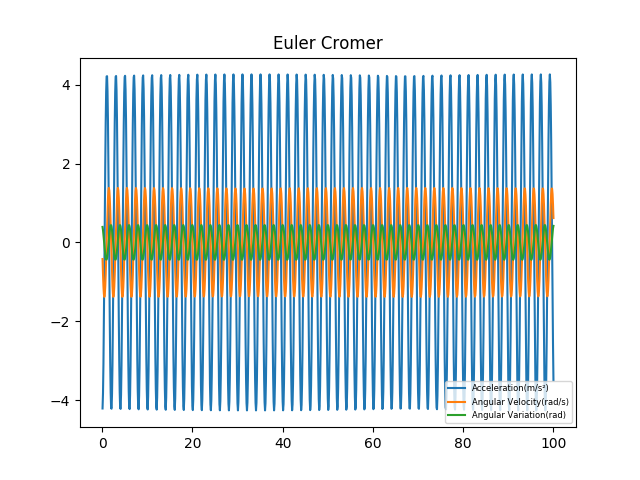
\includegraphics[scale=0.75]{Euler_Cromer_1000.png} \\
$$dt=0.1s\ \text{e}\ 1000\ \text{iterações}$$
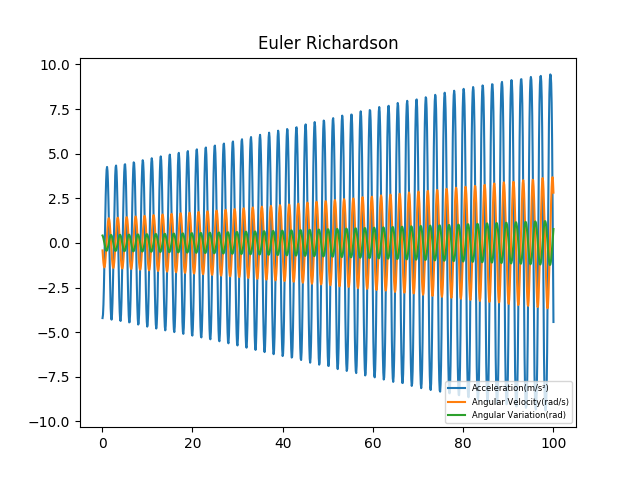
\includegraphics[scale=0.75]{Euler_Richardson_1000.png} \\
$$dt=0.1s\ \text{e}\ 1000\ \text{iterações}$$


\subsection*{Movimento circular uniforme}
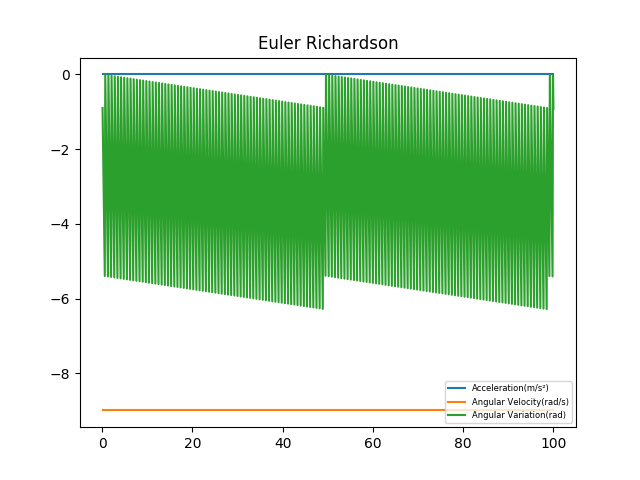
\includegraphics[scale=0.75]{Euler_Cromer_1000_01_MCU.png} \\
$$dt=0.1s\ \text{e}\ 1000\ \text{iterações}$$
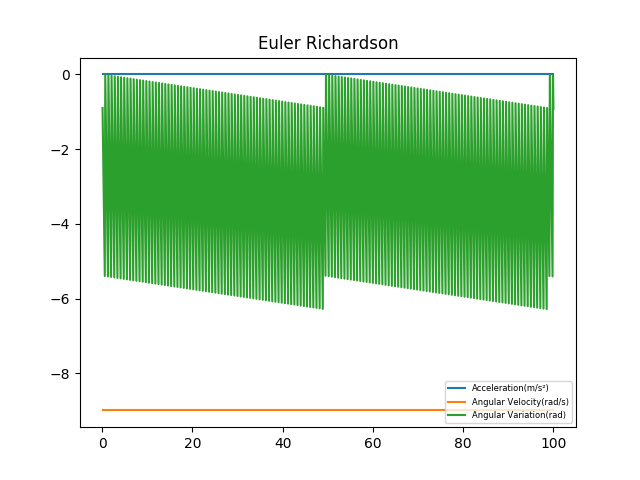
\includegraphics[scale=0.75]{Euler_Richardson_1000_01_MCU.png} \\
$$dt=0.1s\ \text{e}\ 1000\ \text{iterações}$$

\section*{Gráficos}
\subsection*{Pêndulo}
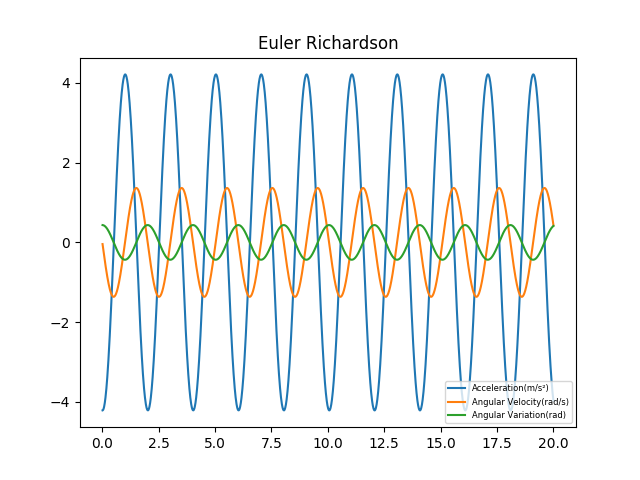
\includegraphics[scale=0.75]{Euler_Cromer.png} \\
$$dt=0.1s\ \text{e}\ 200\ \text{iterações}$$
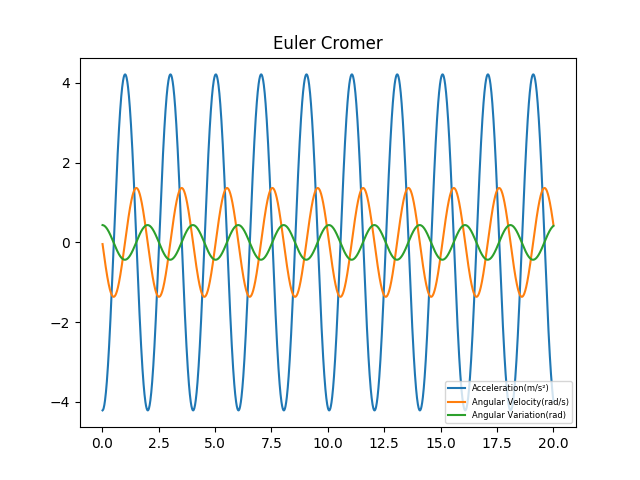
\includegraphics[scale=0.75]{Euler_Richardson.png} \\
$$dt=0.1s\ \text{e}\ 200\ \text{iterações}$$

\subsection*{Movimento circular uniforme}
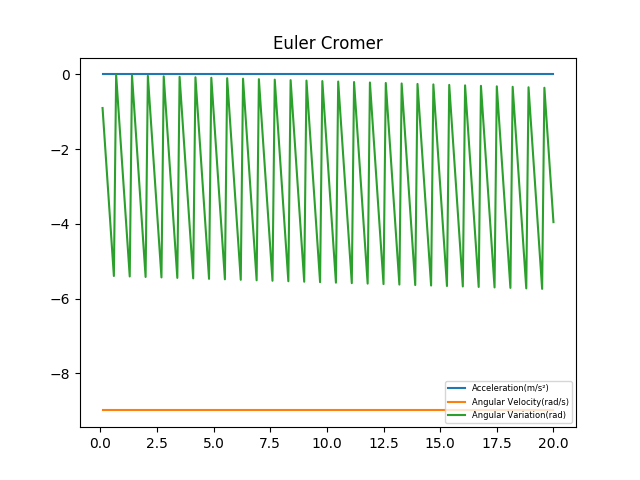
\includegraphics[scale=0.75]{Euler_Cromer_200_01_MCU.png} \\
$$dt=0.1s\ \text{e}\ 200\ \text{iterações}$$
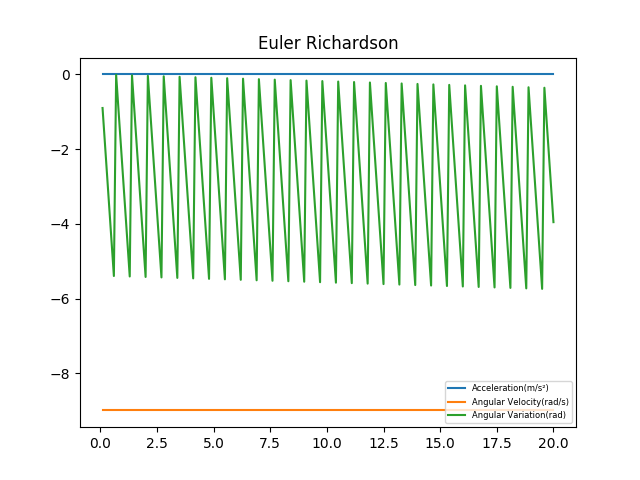
\includegraphics[scale=0.75]{Euler_Richardson_200_01_MCU.png} \\
$$dt=0.1s\ \text{e}\ 200\ \text{iterações}$$


\section*{Análise e interpretação dos gráficos}
\subsection*{Pêndulo}
Os gráficos mostram a oscilação do movimento, e sua repetição em intervalos, 
mostrando as características senóides da velocidade e aceleração. Ambos os 
]algoritmos produziram gráficos idênticos.

\subsection*{Movimento circular uniforme}


\section*{Critícas}
O \textit{Physics Tool Box} possui uma limitação na qual a partir dos 30 
segundos de gravação há um corte de 10 segundos dos dados, isto é, ao chegar
em 30 segundos, a gravação é cortada e só volta a ser resumida perto dos 40
segundos.

\section*{Contribuições}
As contribuições dos membros do grupo em ordem alfabética: \\
\textbf{Beatriz}: Simulações dos movimentos. \\
\textbf{Bruno}: Edição do vídeo.\\
\textbf{João}: Ventilador de teto, simulação dos movimentos.\\
\textbf{Leonardo}: Relatório e EP-relato.\\
\textbf{Lucas}: Coordenação das tarefas e plotting dos dados coletados.\\
\textbf{Victor}: Animações dos plotting.\\

\section*{Link do vídeo}
Para assistir o vídeo, clique
\href{https://youtu.be/roxjSn8T0NI}{aqui}

\end{document}